\documentclass[12pt]{article}
\usepackage{amsmath,amssymb,amsthm}
\usepackage{graphicx,mathabx}
\usepackage{xcolor}
\usepackage{tikz}
\usepackage{cases}
\usepackage{placeins}
\usepackage{lipsum}
\usepackage{mathtools}
\usepackage[shortlabels]{enumitem}
\usepackage{wrapfig}
\DeclarePairedDelimiter{\ceil}{\lceil}{\rceil}
\begin{document}
\title{TCSS 343 - Week 2 - Thursday}
\author{Jake McKenzie}
\maketitle
\noindent\centerline{\textbf{Recurrences and Tracing}}\\\\\\\\\\\\\\\\
\begin{center}
    ``To tell the truth is an act of love. To withhold the truth is an act of hate. Or worse, apathy". \\$\cdots$\\ Gene Kim
\end{center}
\begin{center}
    ``All claims of education notwithstanding, the pupil will accept only that which his mind craves". \\$\cdots$\\ Emma Goldman
\end{center}
\begin{center}
    ``Power concedes nothing without a demand. It never did and it never will". \\$\cdots$\\ Frederick Douglass
\end{center}
\newpage
\begin{enumerate}
\item[0.] The instructions for this problem are in the comments 
lines 1 through 4. \\
\centerline{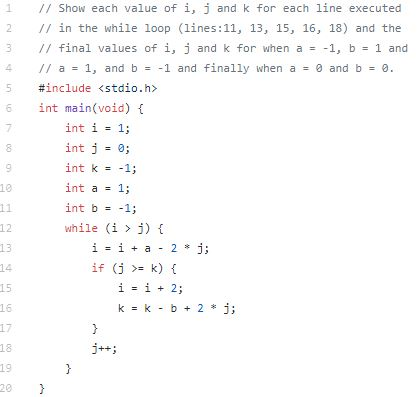
\includegraphics{debug.jpg}} 
\newpage 
\noindent \item Consider the following recurrence:
\begin{numcases}{Z(n)=}
    1, & if $n=1$\\
    3Z(\frac{n}{6}) + n, & $n > 1$
  \end{numcases}
Draw out a visualization of what this recurrences looks like as a tree.\\\\\\\\\\\\\\\\\\\\\\\\\\\\\\\\\\\\\\\\\\\\\\\\\\\\\\\\\\\\
\noindent \item How much work is done on level $i$?
\newpage 
\noindent \item How many recursive levels are there in the tree?\\\\\\\\\\\\\\\\\\\\
\noindent \item How much work is done at the leaf level?\\\\\\\\\\\\\\\\\\\\
\newpage
\noindent \item Construct a non-recursive expression equivalent to the recurrence. Your solution may use a summation.\\\\\\\\\\\\\\\\\\\\
\noindent \item Find the big-$\Theta$ bound for the recurrence.
\newpage 
\noindent \item Consider the following recurrence:
\begin{numcases}{A(n)=}
    1, & if $n=1$\\
    3A(\frac{n}{3}) + 3n^2, & $n > 1$
  \end{numcases}
Draw out a visualization of what this recurrences looks like as a tree.\\\\\\\\\\\\\\\\\\\\\\\\\\\\\\\\\\\\\\\\\\\\\\\\\\\\\\\\\\\\
\noindent \item How much work is done on level $i$?
\newpage 
\noindent \item How many recursive levels are there in the tree?\\\\\\\\\\\\\\\\\\\\
\noindent \item How much work is done at the leaf level?\\\\\\\\\\\\\\\\\\\\
\newpage
\noindent \item Construct a non-recursive expression equivalent to the recurrence. Your solution may use a summation.\\\\\\\\\\\\\\\\\\\\
\noindent \item Find the big-$\Theta$ bound for the recurrence.
\newpage
\noindent \item Write an algorithm Brackets which takes a positive integer n that prints all combinations of well-formed brackets. 
For Brackets(3) the output would be ((())) (()()) (())() ()(()) ()()()
\end{enumerate}
\end{document} 
